\documentclass{article}
\usepackage[utf8]{inputenc}
\usepackage{amsmath}
\usepackage{graphicx}
\usepackage{amsrefs}
\usepackage[a4paper, total={6in, 8in}]{geometry}

\title{Cohort Project 2021, Team 4 \\ Simulating quantum advantage with trapped ions }
\author{}
\date{}

\begin{document}

\maketitle

\section{Introduction}

In 2019 it was announced that the superconducting qubit based quantum computer Sycamore from Google outperformed state-of-the-art classical computers in sampling a pseudo-random quantum circuit probability distribution \cite{Martinis19}.  In this work we perform the same calculation using trapped ion gates simulated on a classical computer.  We explore how the probability distribution depends on the depth (number of layers or gates) and width (number of qubits) of the circuit and how sensitive the resulting speckled pattern is to perturbations (errors in the circuit). 
Next we study the convergence of a perfect quantum random-circuit to a Porter-Thomas distribution and deviations from these distribution as the 2-qubit gate errors increase. 



\section{Task 1: Probability distribution of a quantum random-circuit }

We first simulate the probability distribution if the gates were to be error-free. Even if that would be the case we don't expect the probability distribution to be flat, i.e. every bit-string {\it x} to  appear with the same frequency if the measurement is repeated a large number of times $S$, where $S$ is the number of samples. The reason is that due to quantum interference some bit-strings occur much more often than others, forming a speckled pattern. The computation of such quantum distribution grows exponentially with the number of qubits on a classical computer.

We apply 1 and 2-qubit random gates as in ref. \cite{Martinis19} to entangle the qubits,
\begin{equation}
R(\theta,\varphi)=
\begin{pmatrix}
\cos\frac{\theta}{2} & -ie^{i\varphi}\sin\frac{\theta}{2} \\
-ie \sin\frac{\theta}{2} & \cos\frac{\theta}{2}
\end{pmatrix}
\end{equation}

\begin{equation}
M(\theta)=
\begin{pmatrix}
\cos\Theta & 0& 0& -i\sin\Theta \\
0&\cos\Theta & -i\sin\Theta& 0\\
0 & -i\sin\Theta & \cos\Theta &0 \\
-i\sin\Theta & 0 & 0&\cos\Theta
\end{pmatrix}
\end{equation}
where $R(\theta,\varphi)$ and $M(\theta)$ are gates that can be build with trapped ions.

The probability distribution for different number $N=4,6$ of qubits and depths $3,6,8$ is shown in Fig.\ref{fig:speckled} and exhibits a speckled pattern as expected. Each point represents a  state in Hilbert space,  i.e. one of the possible outcomes of the measurement (bit-string $x$). There are $2^N$ states and the "interference" pattern changes every time we do the sampling.

\begin{figure}[p]
  \centering
  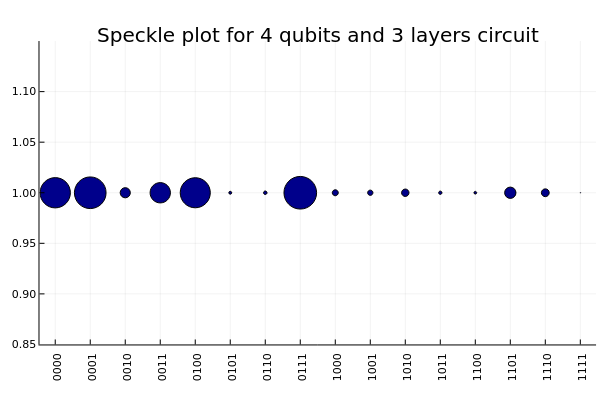
\includegraphics[width=.4\textwidth]{N4_D3_S_1024.png}
  \hspace{1cm}
  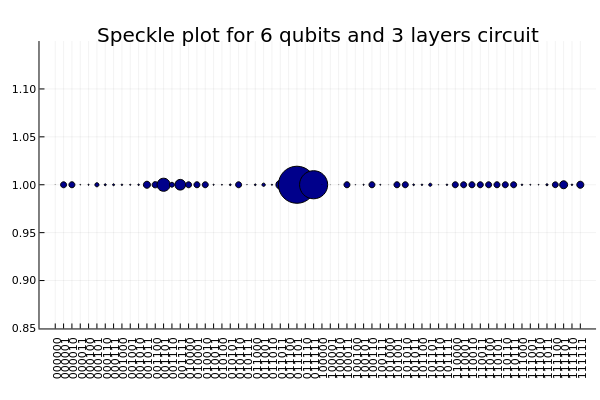
\includegraphics[width=.4\textwidth]{N6_D3_S1024.png}

  \vspace{3cm}

  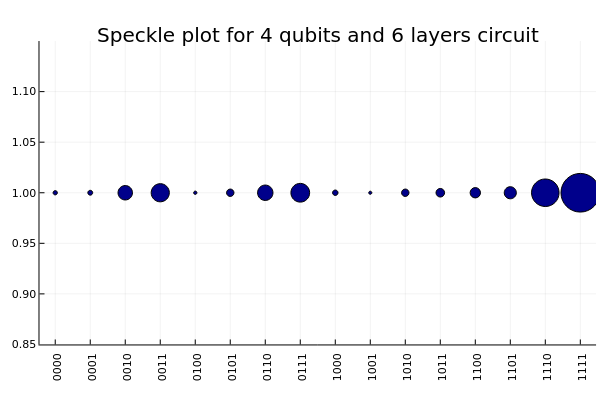
\includegraphics[width=.4\textwidth]{N4_D6_S_1024.png}
  \hspace{1cm}
  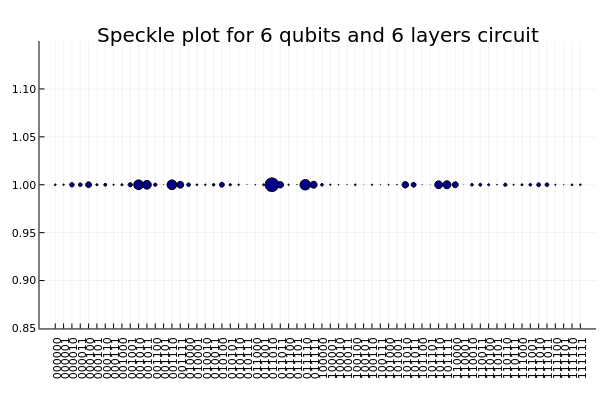
\includegraphics[width=.4\textwidth]{N6_D6_S1024.png}

  \vspace{3cm}

  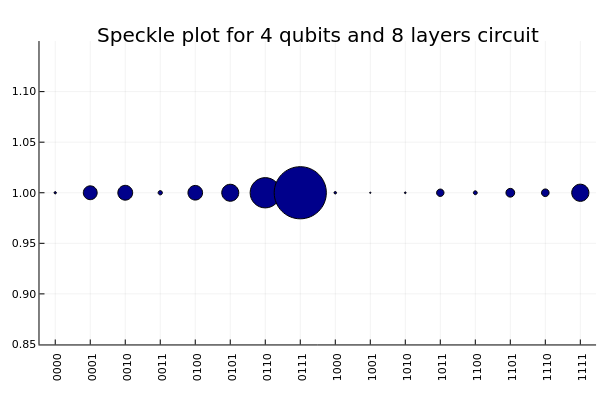
\includegraphics[width=.4\textwidth]{N4_D8_S1024.png}
  \hspace{1cm}
  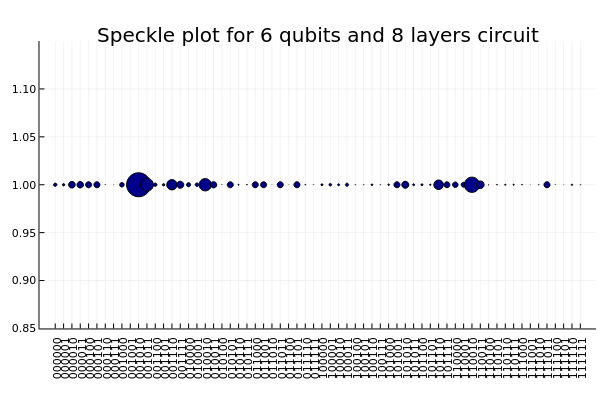
\includegraphics[width=.4\textwidth]{N6_D8_S1024.png}

  \caption{Probability distribution $P(x)=|\langle x|\Psi \rangle|^2$ for a $4$-qubit (left column) and a $6$-qubit (right column) quantum random-circuit of depths =$3,6,8$. The probability is computed from $S=1024$ measurements (shots)}
  \label{fig:speckled}
\end{figure}

%\begin{figure}
 %   \centering
  %  \includegraphics{}
   % \caption{Caption}
    %\label{fig:spackled_pattern}
%\end{figure}
\section{Task 2: Effects of a one spin-flip error at random location}

A large sensitivity to perturbations (i.e. to errors in the application of the gates) is an indication of the emergence of chaos. Here we explore the effects of introducing a perturbation in the form of a spin-flip error, which we model using,
\begin{equation}
\sigma_x=
\begin{pmatrix}
0 & 1 \\
1&0
\end{pmatrix}
\end{equation}

\begin{figure}
    \centering
    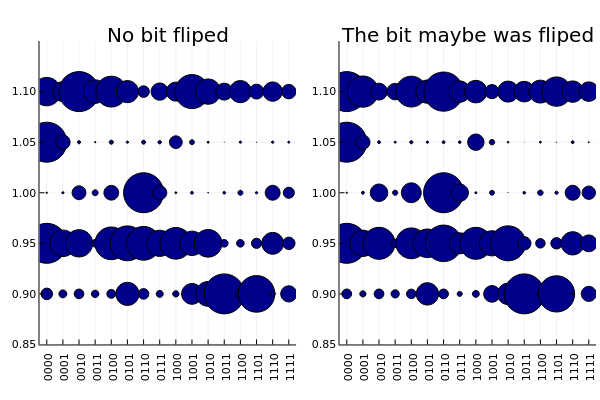
\includegraphics[width=.4\textwidth]{spin_flip.png}
    \caption{Probability distributions from $4$-qubit depth $=4$ random-circuit over  $S=25$ measurements. The left plot shows speckled patterns for the random circuits  without the bit flipped, sampled in different pseudo-experiments, while the right plot displays the speckled patterns using the same parameters as on the left, however now the circuit has a 50 $\%$ chance of one spin being flipped at a random location. }
    \label{fig:spackled_pattern}
\end{figure}

%{\it We observe that for a deep enough random circuit the probability distribution changes drastically depending on the location of the spin-flip  (see Fig.~\ref{fig:spin_flip})} 

\section{Task 3: Convergence to Potter-Thomas distribution}

As the depth of the circuit increases we expect the probability of a given bit-string $x$ to converge to the exponential distribution,
\begin{equation}
    p \rightarrow 2^Ne^{-2Np}
\end{equation}
In Fig.~\ref{fig:PT} we study the convergence of the cumulative distribution $p$ as we increase the depth of the circuit. In the limit of large depth the distribution should converge to a Porter-Thomas distribution \cite{Mullane20}.

\begin{figure}[p]
  \centering
  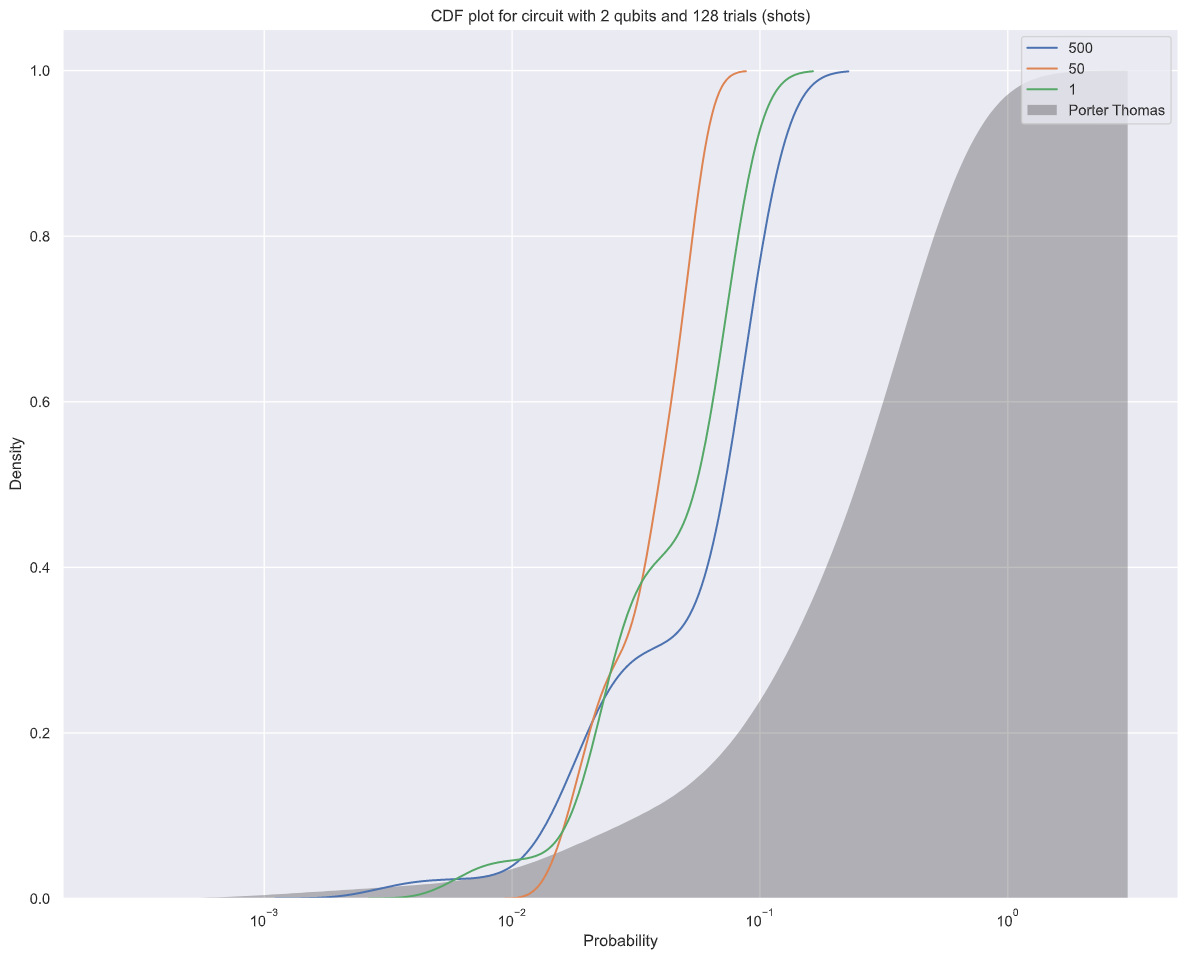
\includegraphics[width=.4\textwidth]{CDF plot for circuit with 2 qubits and 128 trials (shots)}
  \hspace{1cm}
  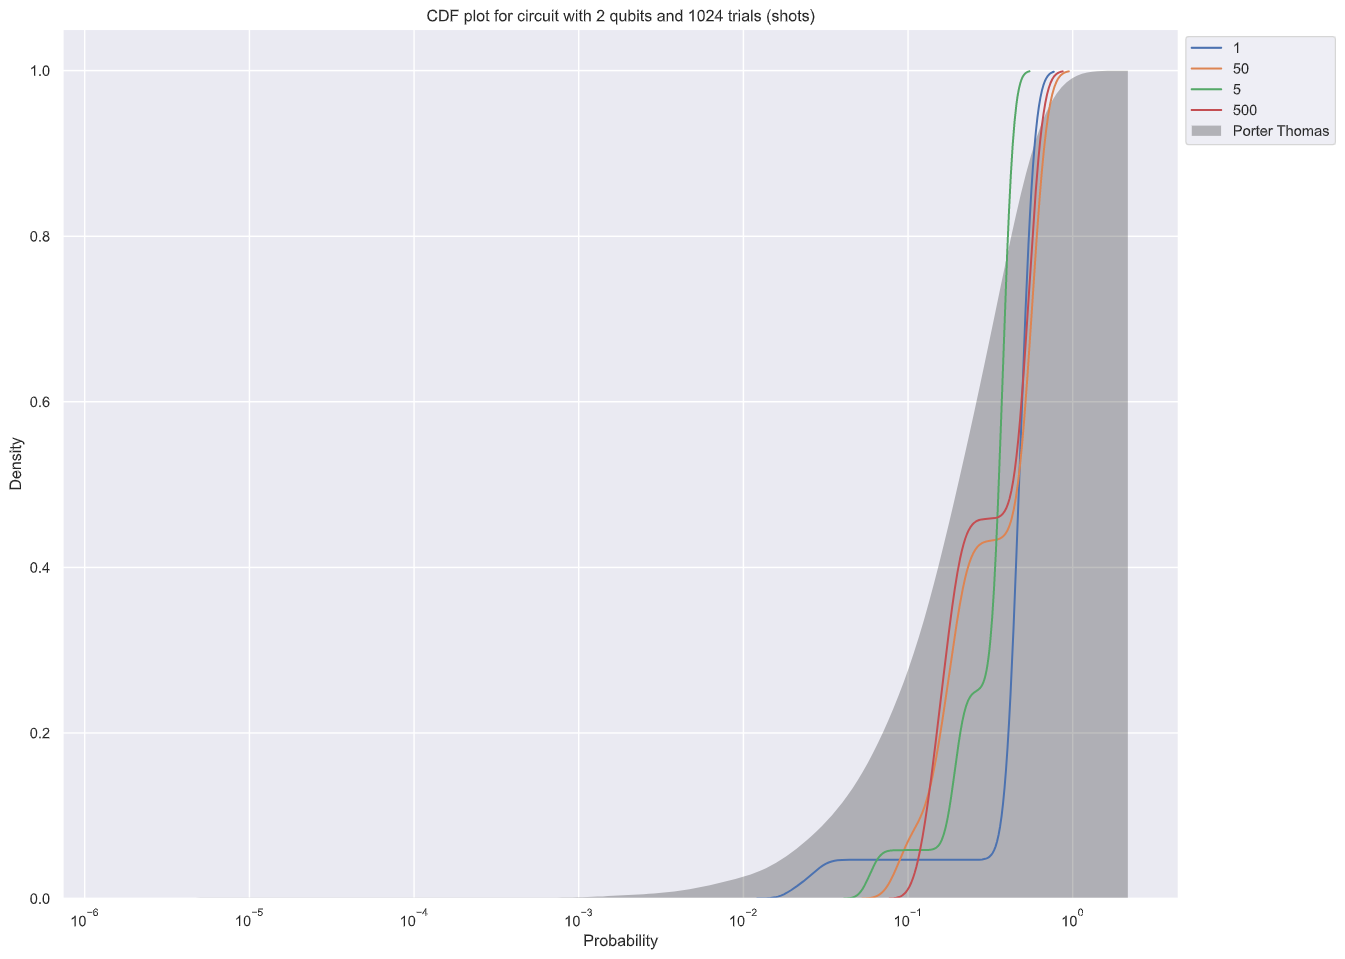
\includegraphics[width=.4\textwidth]{CDF plot for circuit with 2 qubits and 1024 trials (shots)}

  \vspace{3cm}

  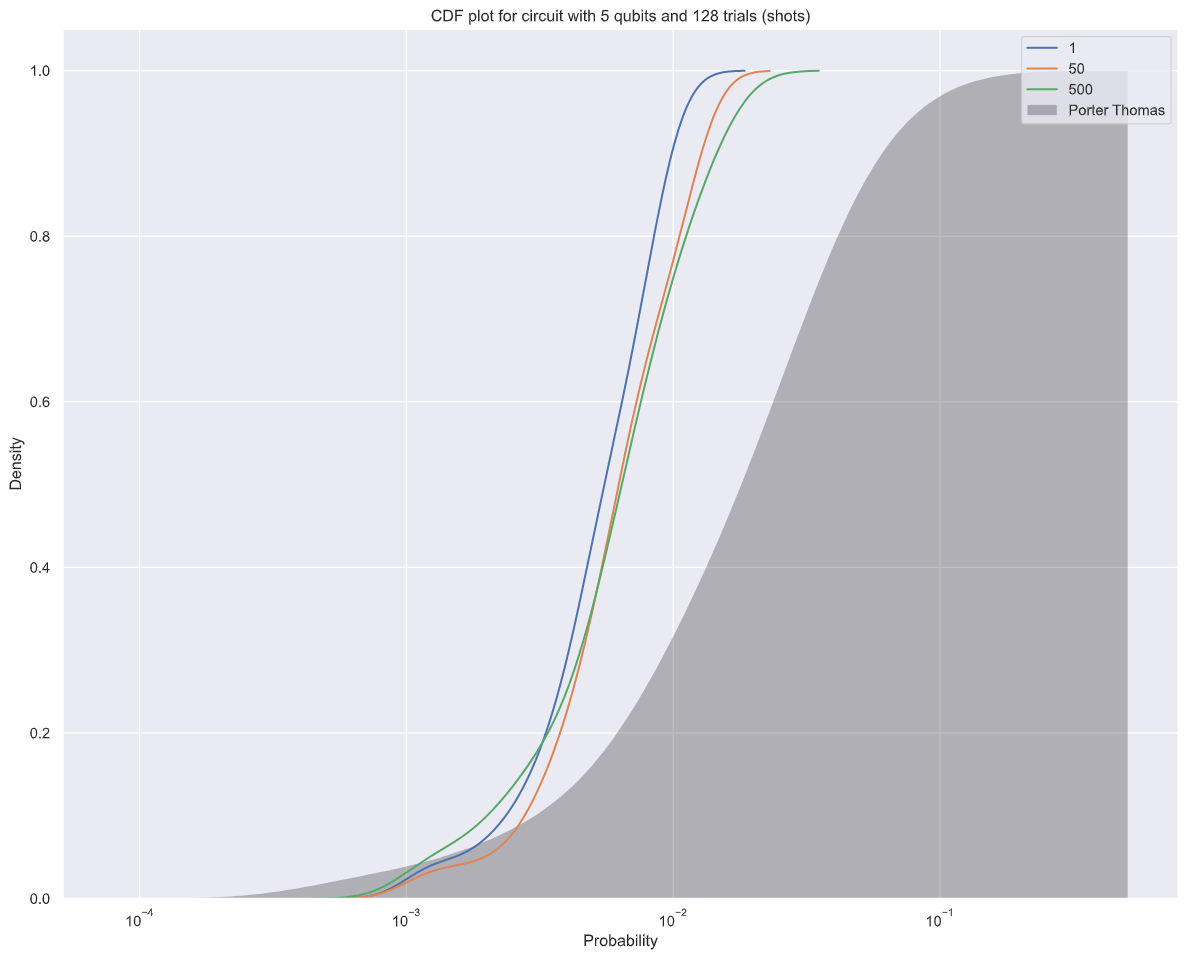
\includegraphics[width=.4\textwidth]{CDF plot for circuit with 5 qubits and 128 trials (shots)}
  \hspace{1cm}
  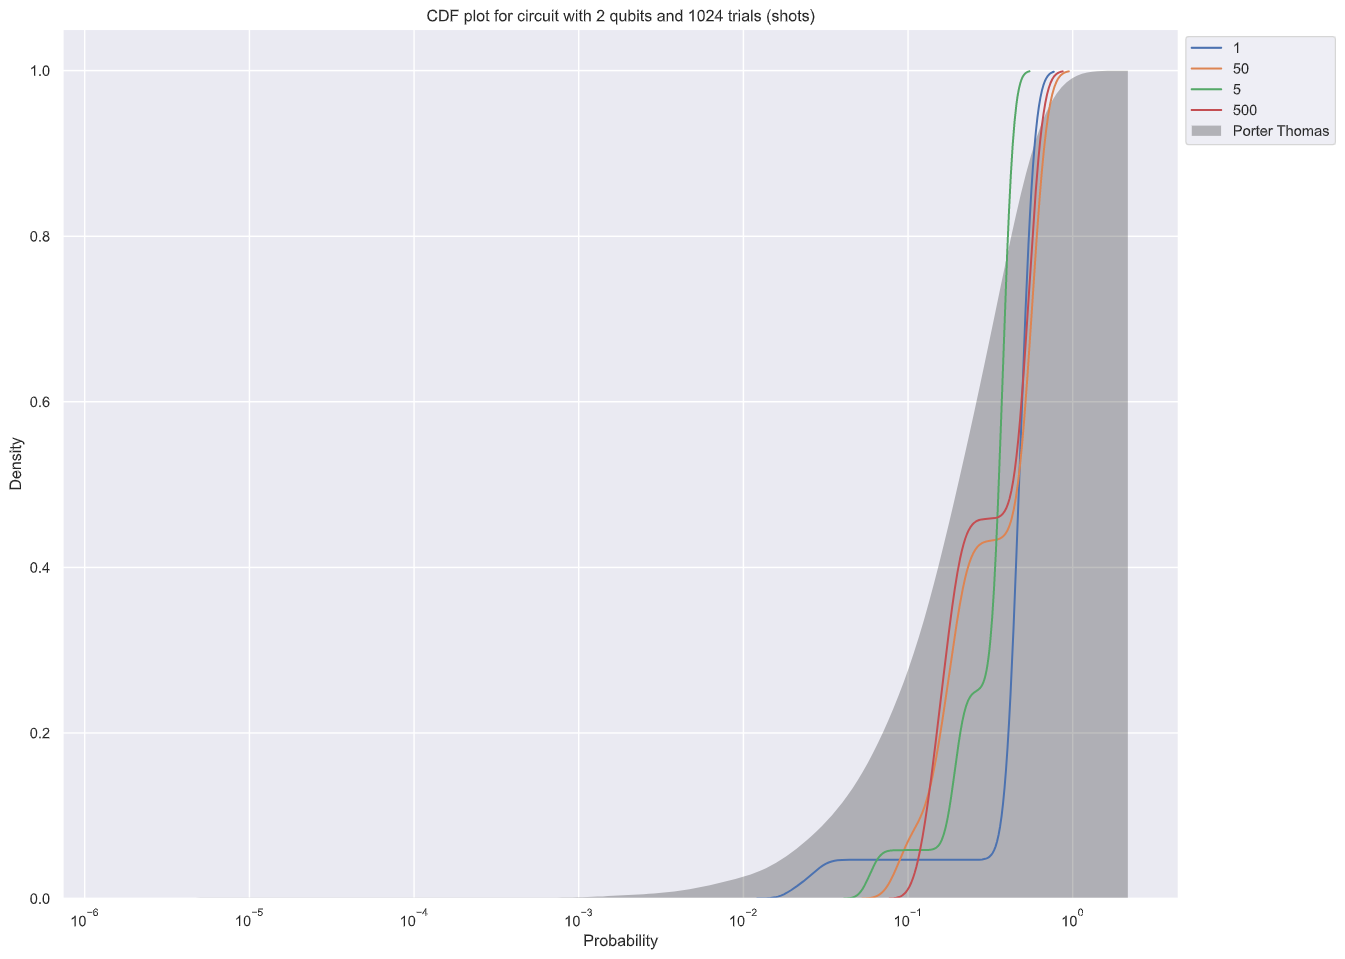
\includegraphics[width=.4\textwidth]{CDF plot for circuit with 2 qubits and 1024 trials (shots)}

  \vspace{3cm}

  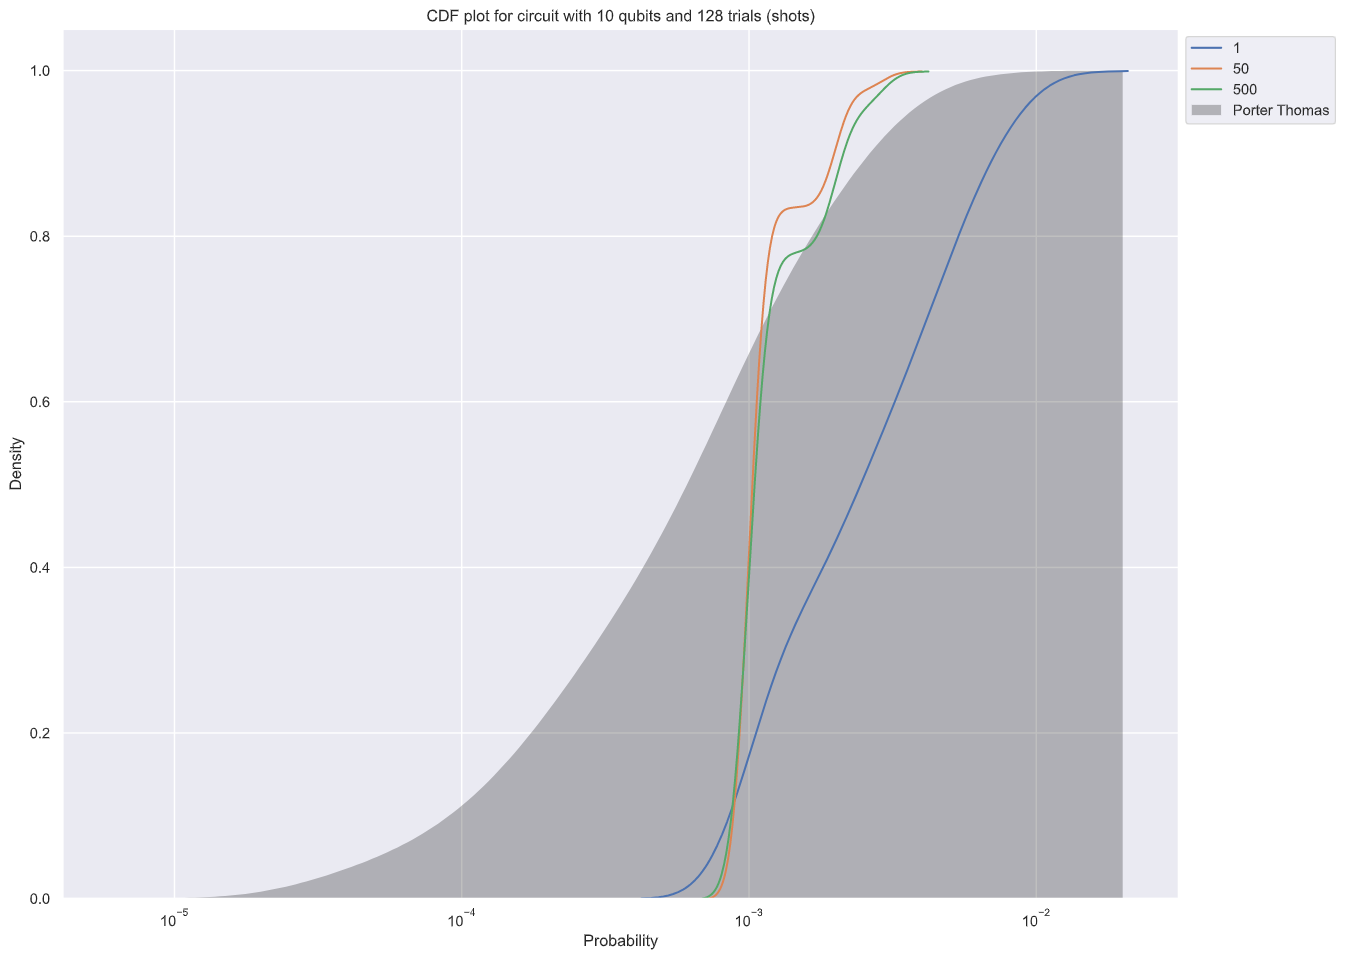
\includegraphics[width=.4\textwidth]{CDF plot for circuit with 10 qubits and 128 trials (shots)}
  \hspace{1cm}
  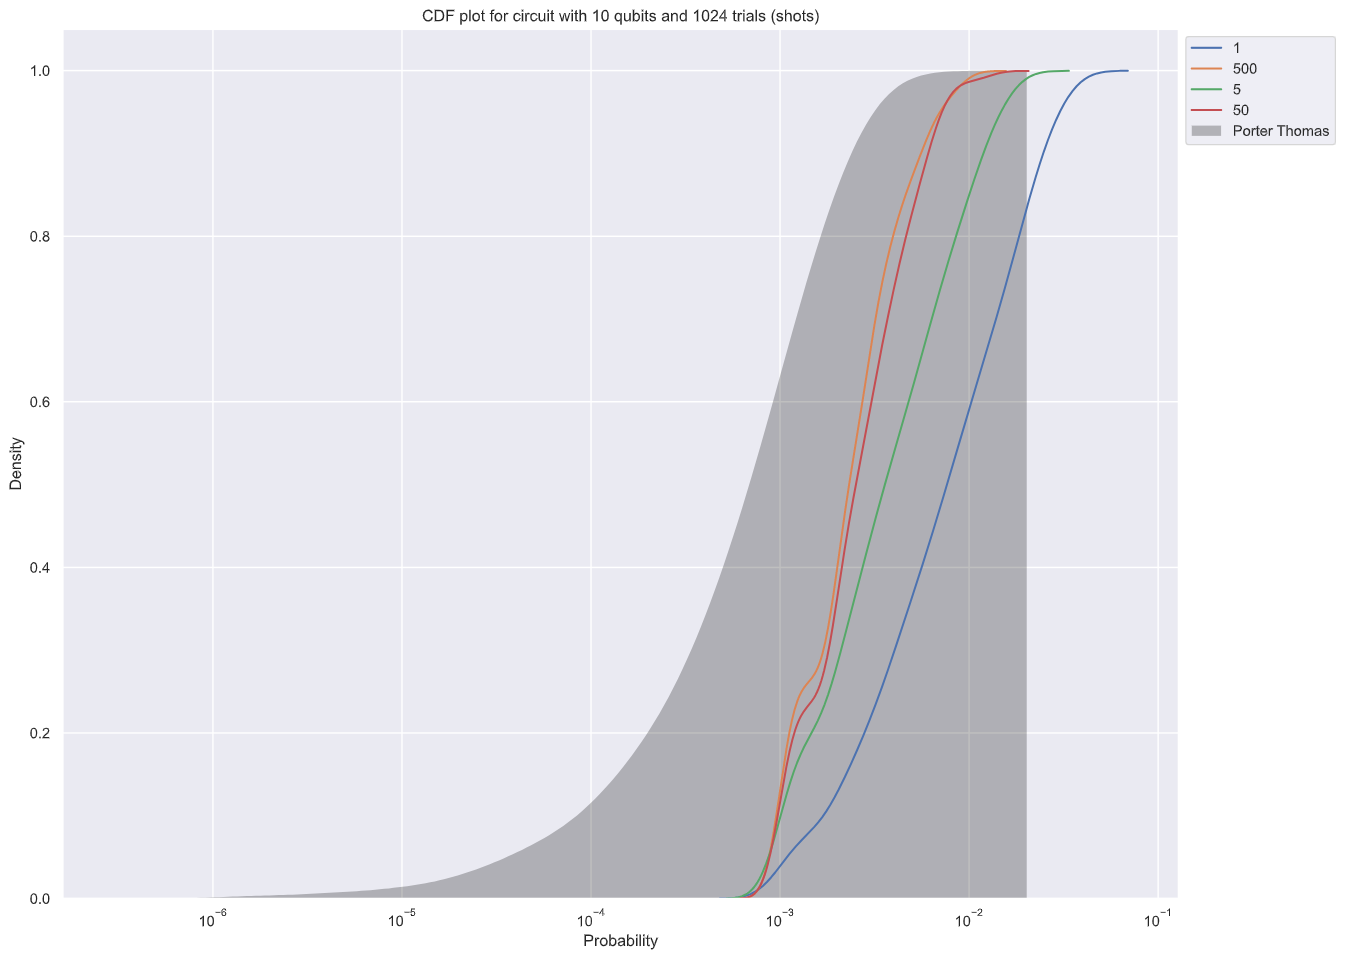
\includegraphics[width=.4\textwidth]{CDF plot for circuit with 10 qubits and 1024 trials (shots)}

  \caption{Cumulative distribution for a $2$-qubit (upper panel) quantum random-circuit of depths =$1,5,50,500$ and $S=128,1024$ (left and right columns respectively). Middle panel: same for a $5$-qubit circuit and lower panel for a $10$-qubit circuit.}
  \label{fig:PT}
\end{figure}

\section{Task 4: Cross-entropy benchmarking fidelity}
An efficient way to assess the quality  of the probability distribution is to compute its 
cross-entropy benchmarking fidelity ${\cal F}_{XEB}$,
\begin{equation}
    {\cal F}_{XEB}=2^N\langle P \rangle -1=\frac{2^N}{S}\sum_{i=1}^SP(x_i) -1
\end{equation}
A uniform distribution where every bit-string $x$ occurs with the same frequency yields ${\cal F}_{XEB}=0$ whereas an error-free quantum random-circuit distribution yields ${\cal F}_{XEB}=1$. A sampling performed on a NISQ quantum computer is therefore expected to yield $0>{\cal F}_{XEB}<1$.
Here we investigate the effect of a sistematic error in the circuit, which we model by perturbing the angle of each 2-qubit gate by a fixed amount $\Delta \Theta$.
{\it}



\section{Supplementary material}
Find in the repo the codes we used to run tasks 1-4.

\begin{bibdiv}
\begin{biblist}
\bib{Martinis19}{article}{
title={Quantum supremacy using a programmable superconducting processor},
author={Arute et al},
journal={Nature},
volume={574},
date={2019},
}
\bib{Mullane20}{article}{
title={Sampling random quantum circuits: a pedestrian’s guide},
author={Mullane, Sean},
date={2020},
url={https://arxiv.org/pdf/2007.07872.pdf}
}

\end{biblist}
\end{bibdiv}


\end{document}

